\chapter{遗传与性状}\label{ch:g9:heredity-and-traits}

家庭照片是生物学数据。外婆的下巴
长在蹒跚学步的孩子脸上，母亲的卷发不见于两个孩子身上，
兄弟二人一高一矮——相似之处在家族中延续，
差异亦然。本书一直借助这一事实，
多年（\cref{rem:g4:animal-reproduction:mix}中的小马驹，
\cref{prop:g8:sexual-reproduction:shuffle}中的兄弟姐妹）；
本学年的开篇一章终于对此展开研究：究竟
什么被\omterm{def:g9:heredity-and-traits:heredity}{遗传}，什么不被\omterm{def:g9:heredity-and-traits:heredity}{遗传}，以及家族
相似性的规律能让我们得出什么结论。

\begin{omfigure}
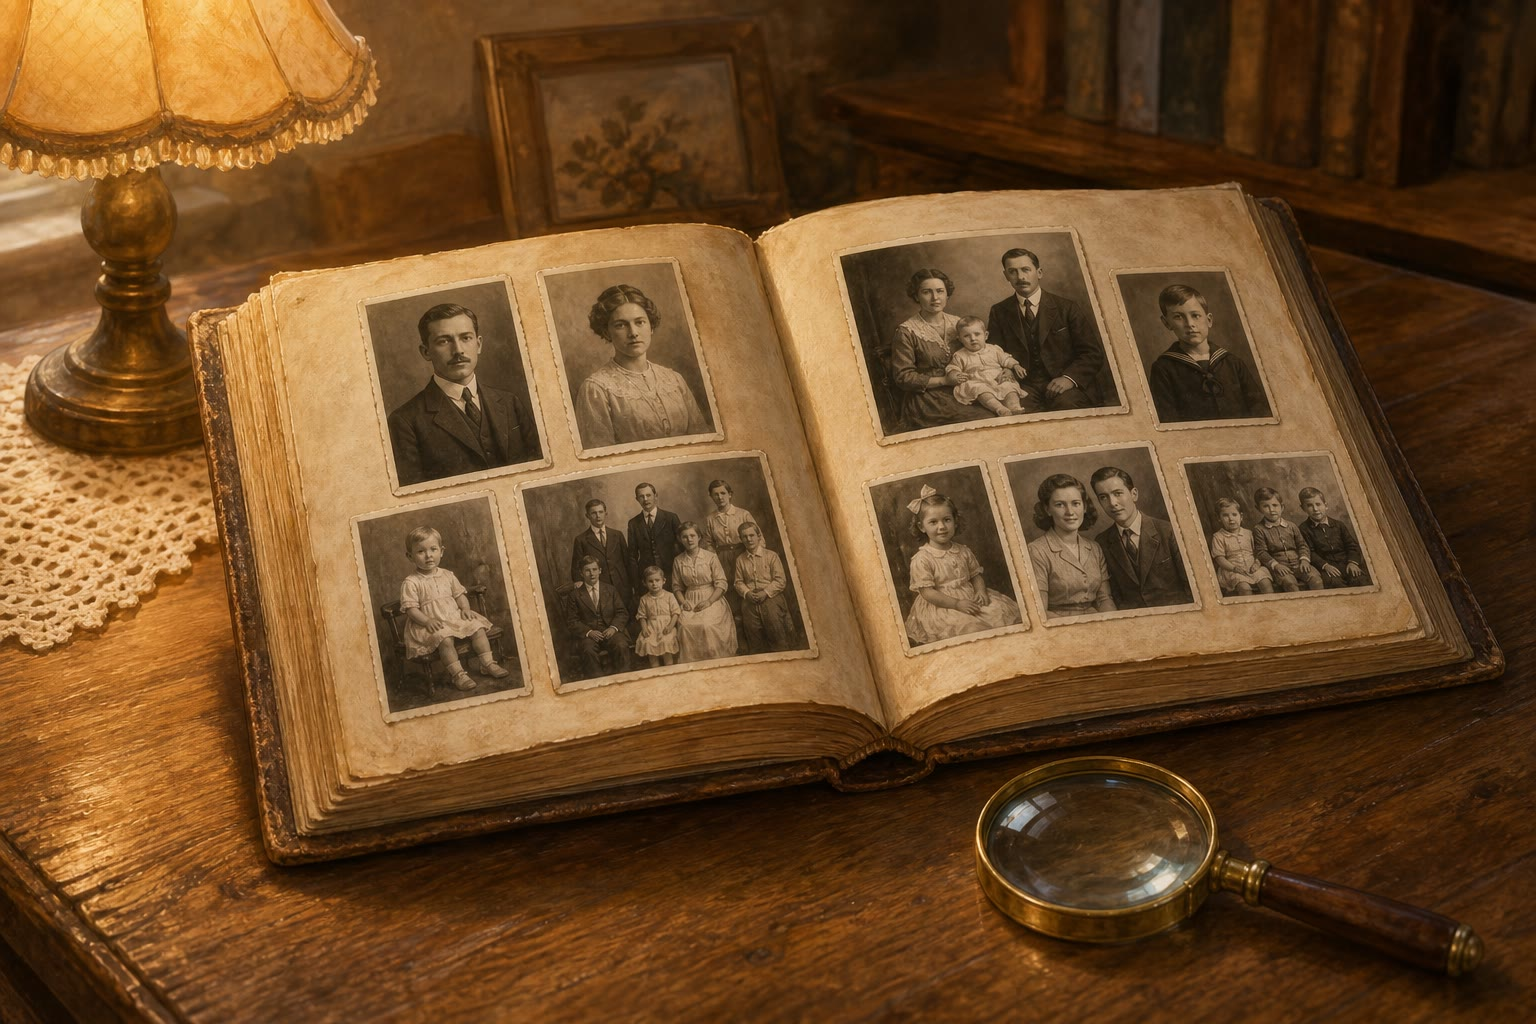
\includegraphics[width=0.62\linewidth]{images/book1/ai/g9-family-album.jpg}

{\small 生物学数据，棕褐色版：相似与
差异，贯穿各代。}
\end{omfigure}

\section{性状及其来源}

\begin{definition}[性状]\label{def:g9:heredity-and-traits:traits}
\emph{性状}\index{性状}是指个体可描述的
任何特征，例如眼睛颜色、血型、
耳垂形状、身高、歌声、疤痕。
个体的全部性状由两种作用形成：
一是\emph{\omterm{def:g9:heredity-and-traits:heredity}{遗传}}所得，二是
\emph{\omterm{def:g6:exploring-our-environment:components}{环境}与生活}所增添的
（\cref{def:g4:adapted-to-their-world:adaptation}中的世界，
作用于同一个身体）。
\end{definition}

\begin{definition}[遗传]\label{def:g9:heredity-and-traits:heredity}
\emph{遗传}\index{遗传}是指\omterm{def:g9:heredity-and-traits:traits}{性状}通过生殖
从亲代传播给后代的过程——
如\cref{ch:g8:sexual-reproduction}所示，经由两个\omterm{def:g6:cell-unit-of-life:unicellular}{单细胞}。
能以此方式传播的\omterm{def:g9:heredity-and-traits:traits}{性状}称为
\emph{遗传性状}\index{遗传性状}：眼睛颜色与
血型属于此类；疤痕与穿耳孔则不属于，无论
佩戴多久。判断的\omterm{def:g3:sorting-living-things:criterion}{标准}是\omterm{def:g8:sexual-reproduction:gametes}{配子}：两个\omterm{def:g5:first-look-at-cells:cell}{细胞}
无法携带的，家族便无法传播。
\end{definition}

\begin{example}[给家庭相册分类]\label{ex:g9:heredity-and-traits:album}
祖父的照片：他那独特的鼻子——
属于\omterm{def:g9:heredity-and-traits:heredity}{遗传}，姑姑和表兄弟身上又见到了；
他那被风吹日晒而成的农家晒黑，属于后天获得，他
坐办公室的孙子就没有这种晒黑；他的身高——部分
是两者兼有，因为孙子在同一张照片中已比他高，
得益于更富足的岁月（见\cref{prop:g3:balanced-diet:jobs}）；
他的小提琴技艺——作为技艺，并不属于\omterm{def:g9:heredity-and-traits:heredity}{遗传}
（\cref{ex:g8:nervous-communication:juggler}：\omterm{def:g8:nervous-communication:synapse}{突触}是经训练形成的，
而非传播而来），不过这个音乐世家
说明在传承的东西中还有更细微的作用，
或许是天赋，而非训练后形成的\omterm{def:g8:nervous-communication:neuron}{神经}连接本身。
\end{example}

\begin{proposition}[遗传的与后天获得的]\label{prop:g9:heredity-and-traits:sorting}
两种作用可以通过三项检验区分：
\begin{enumerate}
  \item \emph{家族模式}：\omterm{def:g9:heredity-and-traits:heredity}{遗传性状}会
        沿生殖的脉络在家谱中反复出现；
        后天获得的\omterm{def:g9:heredity-and-traits:traits}{性状}则随个体的生活而定（所有水手都
        被风吹日晒，不论其父母是谁）；
  \item \emph{起始即在}：血型在\omterm{def:g5:flower-to-fruit:steps}{受精}时
        即已确定；晒黑与技艺则
        在之后形成；
  \item \emph{传播}：截肢者的孩子
        依然生来就有\omterm{def:g1:my-body:parts}{四肢}；健美运动员的孩子
        一出生便不具备训练后的\omterm{def:g3:bones-and-muscles:muscle}{肌肉}。后天获得的\omterm{def:g9:heredity-and-traits:traits}{性状}随
        获得者一同死亡——\omterm{def:g8:sexual-reproduction:gametes}{配子}并不携带它们。
\end{enumerate}
大多数可见的\omterm{def:g9:heredity-and-traits:traits}{性状}——身高、体型，甚至性情——
都由两种作用交织而成：\omterm{def:g9:heredity-and-traits:heredity}{遗传}的范围，以及
生活经历的填充。
\end{proposition}
\admitted

\section{解读家族模式}

\begin{example}[隔代出现的性状]\label{ex:g9:heredity-and-traits:skip}
有些模式乍看令人费解：两位棕色眼睛的
父母生下一个蓝眼睛的孩子；祖母的\omterm{def:g9:heredity-and-traits:traits}{性状}
在每个孩子身上都不见，却在孙辈身上重现。
隔代出现十分常见，它带来一个重要结论：
父母可以\emph{传播自己并不表现出来的东西}。
这一\omterm{def:g9:heredity-and-traits:traits}{性状}的指令在一代之中隐而不显地传递，
所以被\omterm{def:g9:heredity-and-traits:heredity}{遗传}下来的并不是\omterm{def:g9:heredity-and-traits:traits}{性状}本身，而是
某种\emph{决定}该\omterm{def:g9:heredity-and-traits:traits}{性状}的东西，可以在不显现时被携带。
\end{example}

\begin{proposition}[这些模式迫使我们得出的结论]\label{prop:g9:heredity-and-traits:conclusions}
三条结论，每一条都由一项观察所必然导出：
\begin{enumerate}
  \item 既然后天获得的\omterm{def:g9:heredity-and-traits:traits}{性状}不会传递，那么传递下去的
        必定是\emph{决定因子}——即构建\omterm{def:g9:heredity-and-traits:traits}{性状}的指令，
        而非\omterm{def:g9:heredity-and-traits:traits}{性状}本身；
  \item 既然\omterm{def:g9:heredity-and-traits:traits}{性状}会隔代出现，决定因子
        可以在不显现的情况下被\emph{携带}：每个
        个体携带的多于其表现出的。
  \item 既然每个孩子都从双亲各获得一份，
        即借助两个\omterm{def:g8:sexual-reproduction:gametes}{配子}
        （\cref{prop:g8:sexual-reproduction:core}），每位亲代
        贡献其决定因子的一个\emph{选择}，而且
        各个孩子所得的选择彼此不同，
        否则同胞就会完全相同
        （\cref{prop:g8:sexual-reproduction:shuffle}中的洗牌，
        此刻得以定位：这是一种\emph{决定因子}的
        洗牌）。
\end{enumerate}
\end{proposition}
\admitted

\begin{remark}[这一问题的提出]\label{rem:g9:heredity-and-traits:question}
家庭相册把我们引向了一个奇妙的
问题。\omterm{def:g8:reproductive-systems:male}{精子}\omterm{def:g5:first-look-at-cells:cell}{细胞}那几乎微不足道的
（\cref{ex:g8:reproductive-systems:sperm}——一个紧凑的
\omterm{def:g6:cell-unit-of-life:parts}{细胞核}和一条尾巴）里，携带着鼻子、血型、
眼色的指令——可隐而不显地携带，
可按半数挑选，可被生长中的身体读取。
\emph{它们在哪里，又由什么构成？}
\omterm{def:g8:reproductive-systems:male}{精子}的结构已经指明了答案：父亲传递的全部
内容恰好能装进一个\omterm{def:g6:cell-unit-of-life:parts}{细胞核}中
（\cref{rem:g5:first-look-at-cells:nucleus}曾指出，那一部位
很重要）。接下来的两章将打开它。
\end{remark}

\begin{method}[审查一个性状]\label{met:g9:heredity-and-traits:audit}
对任一\omterm{def:g9:heredity-and-traits:traits}{性状}，进行以下三项检验：
\begin{enumerate}
  \item 将其标在家族谱系图上：它是随生殖的谱系传递，
        还是随生活与习惯而来？
  \item 确定其出现时间：从一开始即固定，
        还是在成长过程中逐渐形成？
  \item 进行\omterm{def:g8:sexual-reproduction:gametes}{配子}检验：两个\omterm{def:g8:sexual-reproduction:gametes}{配子}能否携带它？
        （疤痕不能，血型可以）；
  \item 作出判断：\omterm{def:g9:heredity-and-traits:heredity}{遗传}的、获得的，或——最常见的
——\omterm{def:g9:heredity-and-traits:heredity}{遗传}的范围，并在生活中形成。
\end{enumerate}
\end{method}

\section{练习}

\begin{exercise}[$\star$]\label{exo:g9:heredity-and-traits:1}
给出\omterm{def:g9:heredity-and-traits:traits}{性状}与\omterm{def:g9:heredity-and-traits:heredity}{遗传}的定义，并以一句话
说明分类检验。
\end{exercise}

\begin{exercise}[$\star$]\label{exo:g9:heredity-and-traits:2}
对下列各项作出分类：血型；穿耳洞；雀斑；
流利地说法语；耳垂形状。
\end{exercise}

\begin{exercise}[$\star$]\label{exo:g9:heredity-and-traits:3}
说出
\cref{prop:g9:heredity-and-traits:sorting}中的三项检验。
\end{exercise}

\begin{exercise}[$\star$]\label{exo:g9:heredity-and-traits:4}
健美运动员的孩子为何一开始就未经训练？
这说明了什么？
\end{exercise}

\begin{exercise}[$\star$]\label{exo:g9:heredity-and-traits:5}
跳代出现的\omterm{def:g9:heredity-and-traits:traits}{性状}能证明父母能做到什么？
\end{exercise}

\begin{exercise}[$\star$]\label{exo:g9:heredity-and-traits:6}
为什么\omterm{def:g9:heredity-and-traits:heredity}{遗传}下来的必须是决定因子，而不是
\omterm{def:g9:heredity-and-traits:traits}{性状}？请用一句话回答。
\end{exercise}

\begin{exercise}[$\star\star$]\label{exo:g9:heredity-and-traits:7}
同样的体格，孙子长得更高。
请分析这句话中的两种作用机制。
\end{exercise}

\begin{exercise}[$\star\star$]\label{exo:g9:heredity-and-traits:8}
用决定因子的语言解释：为何同胞各不相同——
以及为何同卵双胞胎
（\cref{exo:g8:from-egg-to-birth:10}）却并非如此。
\end{exercise}

\begin{exercise}[$\star\star$]\label{exo:g9:heredity-and-traits:9}
对下列两项运用\cref{met:g9:heredity-and-traits:audit}进行审查：(a) 一个
家庭中反复出现的早白头发；(b) 一名足球
运动员的耐力。
\end{exercise}

\begin{exercise}[$\star\star$]\label{exo:g9:heredity-and-traits:10}
小提琴的例子：若音乐世家传递的从来不是
经过训练的技艺，那么它可能传递的是什么？请
仔细区分。
\end{exercise}

\begin{exercise}[$\star\star$]\label{exo:g9:heredity-and-traits:11}
双亲皆为褐眼，孩子却是蓝眼——邻居
便怀疑这一家庭。请运用
\cref{ex:g9:heredity-and-traits:skip}的逻辑为之辩护。
\end{exercise}

\begin{exercise}[$\star\star\star$]\label{exo:g9:heredity-and-traits:12}
仅从\omterm{def:g8:reproductive-systems:male}{精子}\omterm{def:g5:first-look-at-cells:cell}{细胞}的结构出发，
（\cref{ex:g8:reproductive-systems:sperm}），论证
父亲的决定因子必然位于何处——以及这一结论
对一个完整人类的指令意味着多大的规模。
\end{exercise}

\section{问题：乡村家谱学者}

\begin{problem}[{周末问题——三代人，
一本性状账簿}]\label{pb:g9:heredity-and-traits:1}
一位乡村家谱学者在教区的家谱上
为各家族标注\omterm{def:g9:heredity-and-traits:traits}{性状}：“礼拜堂下巴”（一种独特的
下巴，百年间反复出现）、左利手、
面包师的“面粉肺咳”、取自捐献登记册的血型，
以及牧羊人饱经风霜的面容。

\medskip\noindent\textbf{第一部分——整理
账簿。}
\begin{enumerate}
  \item 依据
        \cref{met:g9:heredity-and-traits:audit}，对五项\omterm{def:g9:heredity-and-traits:traits}{性状}分类，
        并写出每项的决定性检验。
  \item 这种咳嗽跟随面包房而非家族：
        嫁入即带来，迁离即失去。
        这是哪一项检验的实际应用？
  \item “礼拜堂下巴”在
        两个\omterm{def:g1:plants-around-us:tree}{分支}中跳过中间一代。请据此得出它所必然导致的结论。
  \item 血型有时会让登记册感到意外：一个
        A 型与 B 型父母所生的 O 型孩子。
        每位父母各自必须携带了什么？
\end{enumerate}

\medskip\noindent\textbf{第二部分——决定性
读法。}
\begin{enumerate}[resume]
  \item 用决定性语言改写“礼拜堂下巴”的那一世纪：
        沿四代传下去的究竟是什么，
        以何种载体传递
        （\cref{def:g9:heredity-and-traits:heredity}）？
  \item 携带这一下巴特征的表亲，为何
        在其他一切方面都各不相同？请指出其中的重组。
  \item 家谱学家在一个世纪中——未发现一例
        疤痕、手艺或语言传给新生儿的情况——
        请陈述这一概括，
        并说明其机制层面的原因。
  \item 某一家族的双胞胎在下巴乃至更多特征上相符。
        登记册就他们的
        起源作何结论
        （\cref{rem:g5:human-reproduction:twins}）？
\end{enumerate}

\medskip\noindent\textbf{第三部分——讲座。}
\begin{enumerate}[resume]
  \item 家谱学家讲道：“教区传递两种\omterm{def:g9:heredity-and-traits:heredity}{遗传}
        ——一种借助\omterm{def:g8:sexual-reproduction:gametes}{配子}，一种借助
        共同生活。”请把登记册上的五项
        \omterm{def:g9:heredity-and-traits:traits}{性状}分别归入这两条途径。
  \item “我们每个人显露的，少于所携带的。”
        请两次依据登记册加以论证。
  \item 一位听众问，\omterm{def:g8:sexual-reproduction:gametes}{配子}途径所携带的
        “指令”在物理上是什么。请给出
        \cref{rem:g9:heredity-and-traits:question}中的坦诚回答
        ——位置已知，内容留待下一章。
  \item 以审计的一句话结论收束讲座，
        针对最常见的情形：多数\omterm{def:g9:heredity-and-traits:traits}{性状}是
        \emph{什么}，又是\emph{如何}活出来的？
\end{enumerate}
\end{problem}
